\documentclass[11pt,a4paper]{article}
\usepackage[utf8]{inputenc}
\usepackage[T1]{fontenc}
\usepackage{lmodern,amsmath,amssymb,graphicx,booktabs,array,microtype}
\usepackage[margin=22mm]{geometry}
\usepackage[colorlinks=true,linkcolor=blue,urlcolor=blue,citecolor=blue]{hyperref}
\usepackage{fancyhdr}
\pagestyle{fancy}\fancyhf{}\fancyhead[L]{\small Dynagénèse - Épluchage convexe à taille finie}
\fancyhead[R]{\small Complément du 2 novembre 2026}\fancyfoot[C]{\thepage}
\setlength{\headheight}{14pt}
\hypersetup{pdftitle={Anisotropie de reseau a taille finie dans lepluchage convexe},pdfauthor={Patrick Royer},pdfsubject={Residus angulaires, certificats de sauts et prevision conditionnelle}}
\setlength{\parindent}{0pt}\setlength{\parskip}{6pt}
\setlength{\emergencystretch}{2em}
\newcommand{\Rea}{\operatorname{Re}}
\newcommand{\sci}[2]{#1\times10^{#2}}
\newcommand{\R}{\mathbb R}\newcommand{\Z}{\mathbb Z}
\title{\vspace{-14mm}\textbf{Anisotropie de réseau à taille finie dans l'épluchage convexe}\\[3mm]
\large Résidus angulaires, certificats de sauts et prévision conditionnelle à un pas}
\author{Patrick Royer\\\small Chercheur indépendant, non affilié - Dynagénèse}
\date{2 novembre 2026 - Complément scientifique à la publication initiale}
\begin{document}
\maketitle\thispagestyle{fancy}
\vspace{-5mm}
\textbf{Résumé.} Nous étudions les effets du réseau à taille finie dans l'épluchage des seuls sommets stricts d'un ensemble entier convexe. Des trajectoires sauvegardées, issues de 64 translations, deux résolutions et trois orientations d'une forme lisse à symétrie ternaire, sont réanalysées sans ajustement de l'horloge. Des contrôles de rotation et de réflexion reproduisent la géométrie entière attendue. L'intégration angulaire du troisième mode du support révèle des compensations importantes : la localisation d'un petit solde signé ne décrit pas une concentration de sa magnitude absolue. Un certificat causal élémentaire garantit une amplitude d'un niveau entier pour 99,73\,\% des naissances de paliers informatifs, avec abstentions explicites et aucun échec parmi les événements certifiés complets. Deux reconstructions spécifiées à seize directions ne résolvent pas le résidu global à son échelle. À partir du polygone courant complet, une carte exacte à un pas reproduit 1\,152 polygones suivants et leurs contributions de Fourier. Cette carte est une réalisation de l'opérateur microscopique ; elle ne constitue pas une loi macroscopique autonome.

\textbf{Abstract.} We examine finite-scale lattice anisotropy in strict-vertex grid peeling of a smooth, strictly convex, threefold-symmetric planar shape. Existing trajectories at two resolutions and three orientations are analyzed using frozen reference calculations and 64 lattice translations. Rotation and reflection controls reproduce the expected integer geometry. Exact angular integration of the normalized third support mode reveals substantial cancellation between sectors. We derive an elementary causal sufficient condition for the next support drop to equal one primitive lattice level. It certifies 99.73\% of informative plateau births, with explicit abstentions and no failures among completed certified events. Two specified reconstructions from sixteen directional supports fail at the observed residual scale. A column-based one-step map using the complete current polygon reproduces 1,152 saved successor polygons without fitted parameters. This conditional microscopic calculation establishes neither an autonomous macroscopic law nor a continuum convergence theorem.

\section{Question et positionnement}
Le lien entre épluchage de réseau et flot affine de raccourcissement des courbes a déjà fait l'objet d'études expérimentales et théoriques\,\cite{eppstein}. Une convergence et un facteur de temps ont notamment été établis pour une classe de paraboles\,\cite{rote}. Le présent complément porte sur les résidus d'une expérience à résolutions finies, dans le prolongement de la note et du corpus déjà diffusés\,\cite{royer}.

Notre question est limitée : comment une anisotropie directionnelle du procédé discret contribue-t-elle au résidu global signé du troisième mode du support ? Nous distinguons observation rétrospective, certificat géométrique, prévision conditionnelle et évolution autonome. La nouveauté bibliographique précise des règles élémentaires ci-dessous reste à évaluer par une relecture spécialisée.

\newpage
\section{Conventions, corpus et référence}
Le support initial dans le repère de la forme est
\begin{equation}
h_0(\phi)=1-\frac{3}{40}\cos(3\phi),\qquad
\rho_0(\phi)=h_0+h_0''=1+\frac35\cos(3\phi)>0.
\end{equation}
Nous utilisons les 64 translations dyadiques figées de la campagne initiale, de dénominateur $2^{20}$, les résolutions $R=256,512$, et les orientations $\theta\in\{0,\arctan(1/8),\pi/4\}$. Les analyses du présent complément ont été conçues après examen du corpus : elles sont rétrospectives, même lorsque des prévisions sont produites sans consulter l'état futur dans leur phase de calcul.

Les coordonnées physiques sont $(v+t)/R$, avec $v\in\Z^2$. Si $P_n$ est le polygone entier courant, l'état suivant est l'enveloppe des points présents après retrait de ses seuls sommets extrêmes stricts. Les points colinéaires non extrêmes sont conservés. L'ensemble initial est saturé dans son enveloppe entière, propriété conservée par ces retraits : un sommet retiré ne peut pas se trouver dans l'enveloppe des points restants.

Pour une normale entière primitive $u$, posons
\begin{equation}
k_n(u)=\max_{v\in P_n}u\cdot v,\qquad
H_n(u)=\frac{k_n(u)+u\cdot t}{R\|u\|}.
\end{equation}
L'horloge antérieure reste fixée :
\begin{equation}
t_n=\alpha\,n/R^{4/3},\qquad \alpha=0{,}6450983601211226.
\end{equation}
Les analyses de déplacement comparent les supports bruts à ce temps. Les comparaisons de forme à contraction égale emploient une autre sélection de référence : la cible historique $q$ correspond à
\begin{equation}
c_0^{\mathrm{cible}}=q\,c_{0,\mathrm{initial}},\qquad q\in\{0{,}95,0{,}90,0{,}85\}.
\end{equation}
Le poids d'interpolation de Minkowski entre deux couches adjacentes est calculé sur les coefficients bruts ; la normalisation est appliquée ensuite.

Pour $\phi=\arg(u)-\theta$, définissons
\begin{equation}
c_m=\frac1{2\pi}\int_0^{2\pi}h(\phi)e^{-im\phi}\,d\phi,
\quad a_m=c_m/c_0,\quad c_0=P/(2\pi),
\end{equation}
où $P$ est le périmètre physique. Le passage au repère de la forme multiplie le coefficient global par $e^{im\theta}$, sans phase ajustée. Le résidu étudié est
\begin{equation}
r_3=\Rea\!\left(a_3^{\mathrm{discret}}-a_3^{\mathrm{affine}}\right).
\end{equation}
Il diffère du contraste de pertes $D$ entre exposants utilisé dans la publication initiale. Le signe de $r_3$ ne fournit donc pas, à lui seul, une préférence entre ces exposants.

La référence complète est reconstruite depuis les polynômes BDF sauvegardés ; aucune nouvelle intégration d'EDP n'est effectuée. L'écart déjà qualifié entre ce mode affine et celui de la campagne est au plus $\sci{3{,}73725}{-12}$ aux cibles. Il n'est ni supprimé ni ajusté.

\newpage
\section{Symétries et résidu angulaire}
Une rotation de $90^\circ$ du réseau et la symétrie ternaire de la forme relient $\theta=\pi/4$ à $\pi/12$, avec transformation correspondante de la translation. Les réflexions imposent aussi les conjugaisons de Fourier attendues. Douze paires de contrôles, sur trois translations et deux résolutions, donnent 7\,670 comparaisons de couches avec égalité exacte des ensembles de sommets entiers. Ce contrôle fini n'exclut pas tous les biais qui préserveraient les mêmes symétries.

La direction $\pi/4$ est la direction rationnelle de vecteur primitif $(1,1)$. La norme $\sqrt2$ intervient dans l'espacement physique des lignes du réseau ; l'irrationalité de cette norme n'est pas une explication du résidu. Aucune résonance n'est établie par les résultats présents.

Pour la localisation, le support est recentré par son mode 1 puis divisé par $c_0$. Le recentrage ne modifie pas le mode 3 global, mais modifie ses contributions sur des fenêtres finies. La densité signée est intégrée analytiquement sur les cônes normaux des polygones et sur la référence spectrale complète. Les fenêtres primaires sont $0^\circ\pm5^\circ$ et $180^\circ\pm5^\circ$ dans le repère de la forme ; à $\theta=\pi/4$, leurs centres correspondent à $45^\circ$ et $225^\circ$ dans le réseau.

\begin{table}[h]
\centering\small
\caption{Moyennes sur 64 translations à $\theta=\pi/4$, $R=512$. Valeurs multipliées par $10^6$. Les cibles sont interpolées, et non les couches entières du crochet supérieur.}
\begin{tabular}{rrrrr}\toprule
$q$ & $r_3$ global & Fenêtre $0^\circ$ & Fenêtre $180^\circ$ & Reste\\\midrule
0,95 & $+14{,}1587$ & $+29{,}2540$ & $-15{,}2645$ & $+0{,}1692$\\
0,90 & $-231{,}1500$ & \multicolumn{2}{c}{$-8{,}1253$ (somme des fenêtres)} & $-223{,}0247$\\
0,85 & $-282{,}2584$ & \multicolumn{2}{c}{$+3{,}7474$ (somme des fenêtres)} & $-286{,}0058$\\\bottomrule
\end{tabular}
\end{table}

À $q=0{,}95$, la somme des fenêtres représente environ 99\,\% du petit solde global. Cela ne mesure pas la concentration de la magnitude absolue. L'intégrale de la valeur absolue de la densité moyenne vaut environ $\sci{5{,}259}{-4}$, soit 37 fois le solde. Le rapport net des fenêtres varie aussi avec leur demi-largeur : environ 101\,\%, 99\,\% et 62\,\% pour $2{,}5^\circ$, $5^\circ$ et $10^\circ$.

La dépendance en résolution est essentielle. À $R=256$, les trois résidus moyens correspondants restent positifs : $\sci{2{,}86744}{-4}$, $\sci{2{,}34908}{-4}$ et $\sci{2{,}85782}{-4}$. À $R=512$, le résidu à $q=0{,}95$ est positif dans 57 configurations sur 64, puis les moyennes deviennent négatives aux deux contractions suivantes.

Les analyses de déplacement brut établissent par ailleurs un retard par rapport à la référence à horloge gelée dans les deux directions opposées suivies à $\pi/4$, aux deux résolutions et sur les 64 translations, pendant l'intervalle $0{,}02\le t\le0{,}04$. Le retrait de l'écart initial constant ne le supprime pas. Cela ne réfute pas toute forme possible de mémoire transportée, ni toute erreur anisotrope d'horloge.

\newpage
\section{Un certificat causal d'amplitude}
Fixons une normale primitive $u$, et considérons la naissance d'un niveau supérieur $k$. Soit $m$ le nombre de points présents sur sa face exposée. Ses deux extrémités sont retirées à chaque transition, puis son dernier point lorsqu'il est seul. La première disparition de cette face survient donc après
\begin{equation} L=\lceil m/2\rceil.\end{equation}
Sur la droite immédiatement inférieure $u\cdot x=k-1$, soient $M$ le nombre de points actuellement présents et $r_0$ le nombre de sommets stricts actuels qui s'y trouvent.

\textbf{Proposition (condition suffisante).} Si
\begin{equation}\label{eq:cert}M>r_0+2(L-1),\end{equation}
alors la première baisse de niveau est exactement $\Delta k=1$, après $L$ transitions. Son amplitude physique est
\begin{equation}\Delta H=\frac{1}{R\|u\|}.\end{equation}

\textit{Preuve.} La première transition retire exactement $r_0$ points de la droite inférieure. Une droite ne peut porter plus de deux sommets extrêmes stricts d'un ensemble plan ; chaque transition suivante y retire donc au plus deux points. La condition~\eqref{eq:cert} garantit un survivant sur $k-1$ lorsque la face $k$ disparaît, exactement à la transition $L$. Le prochain support est donc $k-1$.\hfill$\square$

Cette preuve emploie les points réellement présents. Elle ne requiert pas à elle seule la saturation. Dans notre calcul, la saturation permet d'obtenir $m$, $M$ et l'état suivant depuis le seul polygone. Cette distinction précise certaines formulations plus restrictives des bilans techniques antérieurs, dont les archives restent inchangées.

\begin{table}[h]\centering\small
\caption{Certificat renforcé sur les naissances jusqu'au crochet supérieur de $q=0{,}95$. Les événements censurés dépassent l'horizon sauvegardé.}
\begin{tabular}{lrrrr}\toprule
Population & Naissances & Certifiées & Complètes & Censurées\\\midrule
Informative, $m\ge3$ & 263\,364 & 262\,661 & 258\,077 & 4\,584\\
Triviale, $m\le2$ & 286\,512 & 286\,512 & 284\,973 & 1\,539\\
Total & 549\,876 & 549\,173 & 543\,050 & 6\,123\\\bottomrule
\end{tabular}
\end{table}

Aucun événement certifié complet n'échoue. Les 703 abstentions informatives, dont 682 complètes, sont toutes à $R=256$, $\theta=\arctan(1/8)$. À $\pi/4$, toutes les naissances suivies dans les seize directions et les deux résolutions sont certifiées. Les 543\,732 baisses complètes observées, y compris après abstention, sont unitaires ; les cas sans certificat ne sont pas comptés comme prévisions réussies.

Le certificat initial plus conservateur $M>2L$ est conservé dans les suppléments. Le renforcement~\eqref{eq:cert} a été choisi après examen de sa couverture. Aucun coefficient n'est ajusté, mais ce choix n'est pas prospectivement préenregistré. Les événements d'une trajectoire sont dépendants et ne constituent pas autant de réplications statistiques indépendantes.

\newpage
\section{Transfert angulaire et carte conditionnelle}
Connaître l'amplitude dans une normale isolée ne donne pas l'étendue angulaire de son influence. Pour un pas complet, notons $d(\phi)=h_n(\phi)-h_{n+1}(\phi)\ge0$, et
\begin{equation}
J_m=\frac{1}{2\pi}\int d(\phi)e^{-im\phi}\,d\phi.
\end{equation}
Alors $\Delta c_m=-J_m$, et la variation normalisée exacte est
\begin{equation}\label{eq:delta}
\Delta a_3=\frac{-J_3+a_{3,n}J_0}{c_{0,n}-J_0}
=\frac{\Delta c_3-a_{3,n}\Delta c_0}{c_{0,n+1}}.
\end{equation}
Le terme de normalisation ne peut pas être omis. Pour une interpolation de poids $w$ vers une cible $q_{\rm abs}$, la variation normalisée jusqu'à la cible est $w c_{0,n+1}/q_{\rm abs}$ fois celle du pas complet ; elle n'est généralement pas $w\Delta a_3$.

Nous évaluons une carte conditionnelle qui reçoit le polygone entier courant. Pour chaque abscisse entière, elle calcule l'intervalle d'ordonnées entières intérieur au polygone, retire les sommets stricts actuels, puis conserve les extrémités survivantes. L'enveloppe convexe de ces extrémités est exactement celle de tous les points survivants : les autres points sont sur les segments verticaux entre elles. Les sommets stricts sont aux extrémités de leurs colonnes ; leur retrait ne crée pas de trou intérieur. Les prédicats et arrondis sont calculés en entiers Python.

Les données de construction et le benchmark futur sont séparés. Le replay écrit les prévisions et leurs empreintes avant de charger ce benchmark. L'état courant est néanmoins le crochet inférieur d'une cible déjà repérée dans une trajectoire sauvegardée : sa sélection est rétrospective. Ni cet état ni son temps d'atteinte ne sont prévus depuis le début.

\begin{table}[h]\centering\small
\caption{Contrôles de la carte à un pas : 1\,152 cibles, 384 configurations. Les erreurs désignent l'accord avec les sorties discrètes sauvegardées.}
\begin{tabular}{lr}\toprule
Contrôle & Résultat\\\midrule
Polygones entiers conformes & 1\,152 / 1\,152\\
Écarts de nombre de points survivants & 0\\
Erreur maximale de $a_3$ (calcul de référence) & $\sci{2{,}363}{-16}$\\
Erreur maximale de $a_3$ (replay Windows) & $\sci{2{,}159}{-16}$\\
Fermeture angulaire (replay Windows) & $\sci{8{,}080}{-17}$\\\bottomrule
\end{tabular}
\end{table}

Une quadrature indépendante, sans importer l'intégrateur du prédicteur, contrôle 48 polygones sur 24 cibles : l'erreur maximale sur le mode cible est $\sci{1{,}46}{-16}$. Les polygones, coefficients et contributions angulaires ont aussi été reproduits dans l'environnement Windows de l'auteur. Ce replay de la même méthode et des mêmes données n'est pas une confirmation statistique indépendante.

\newpage
\begin{figure}[p]\centering
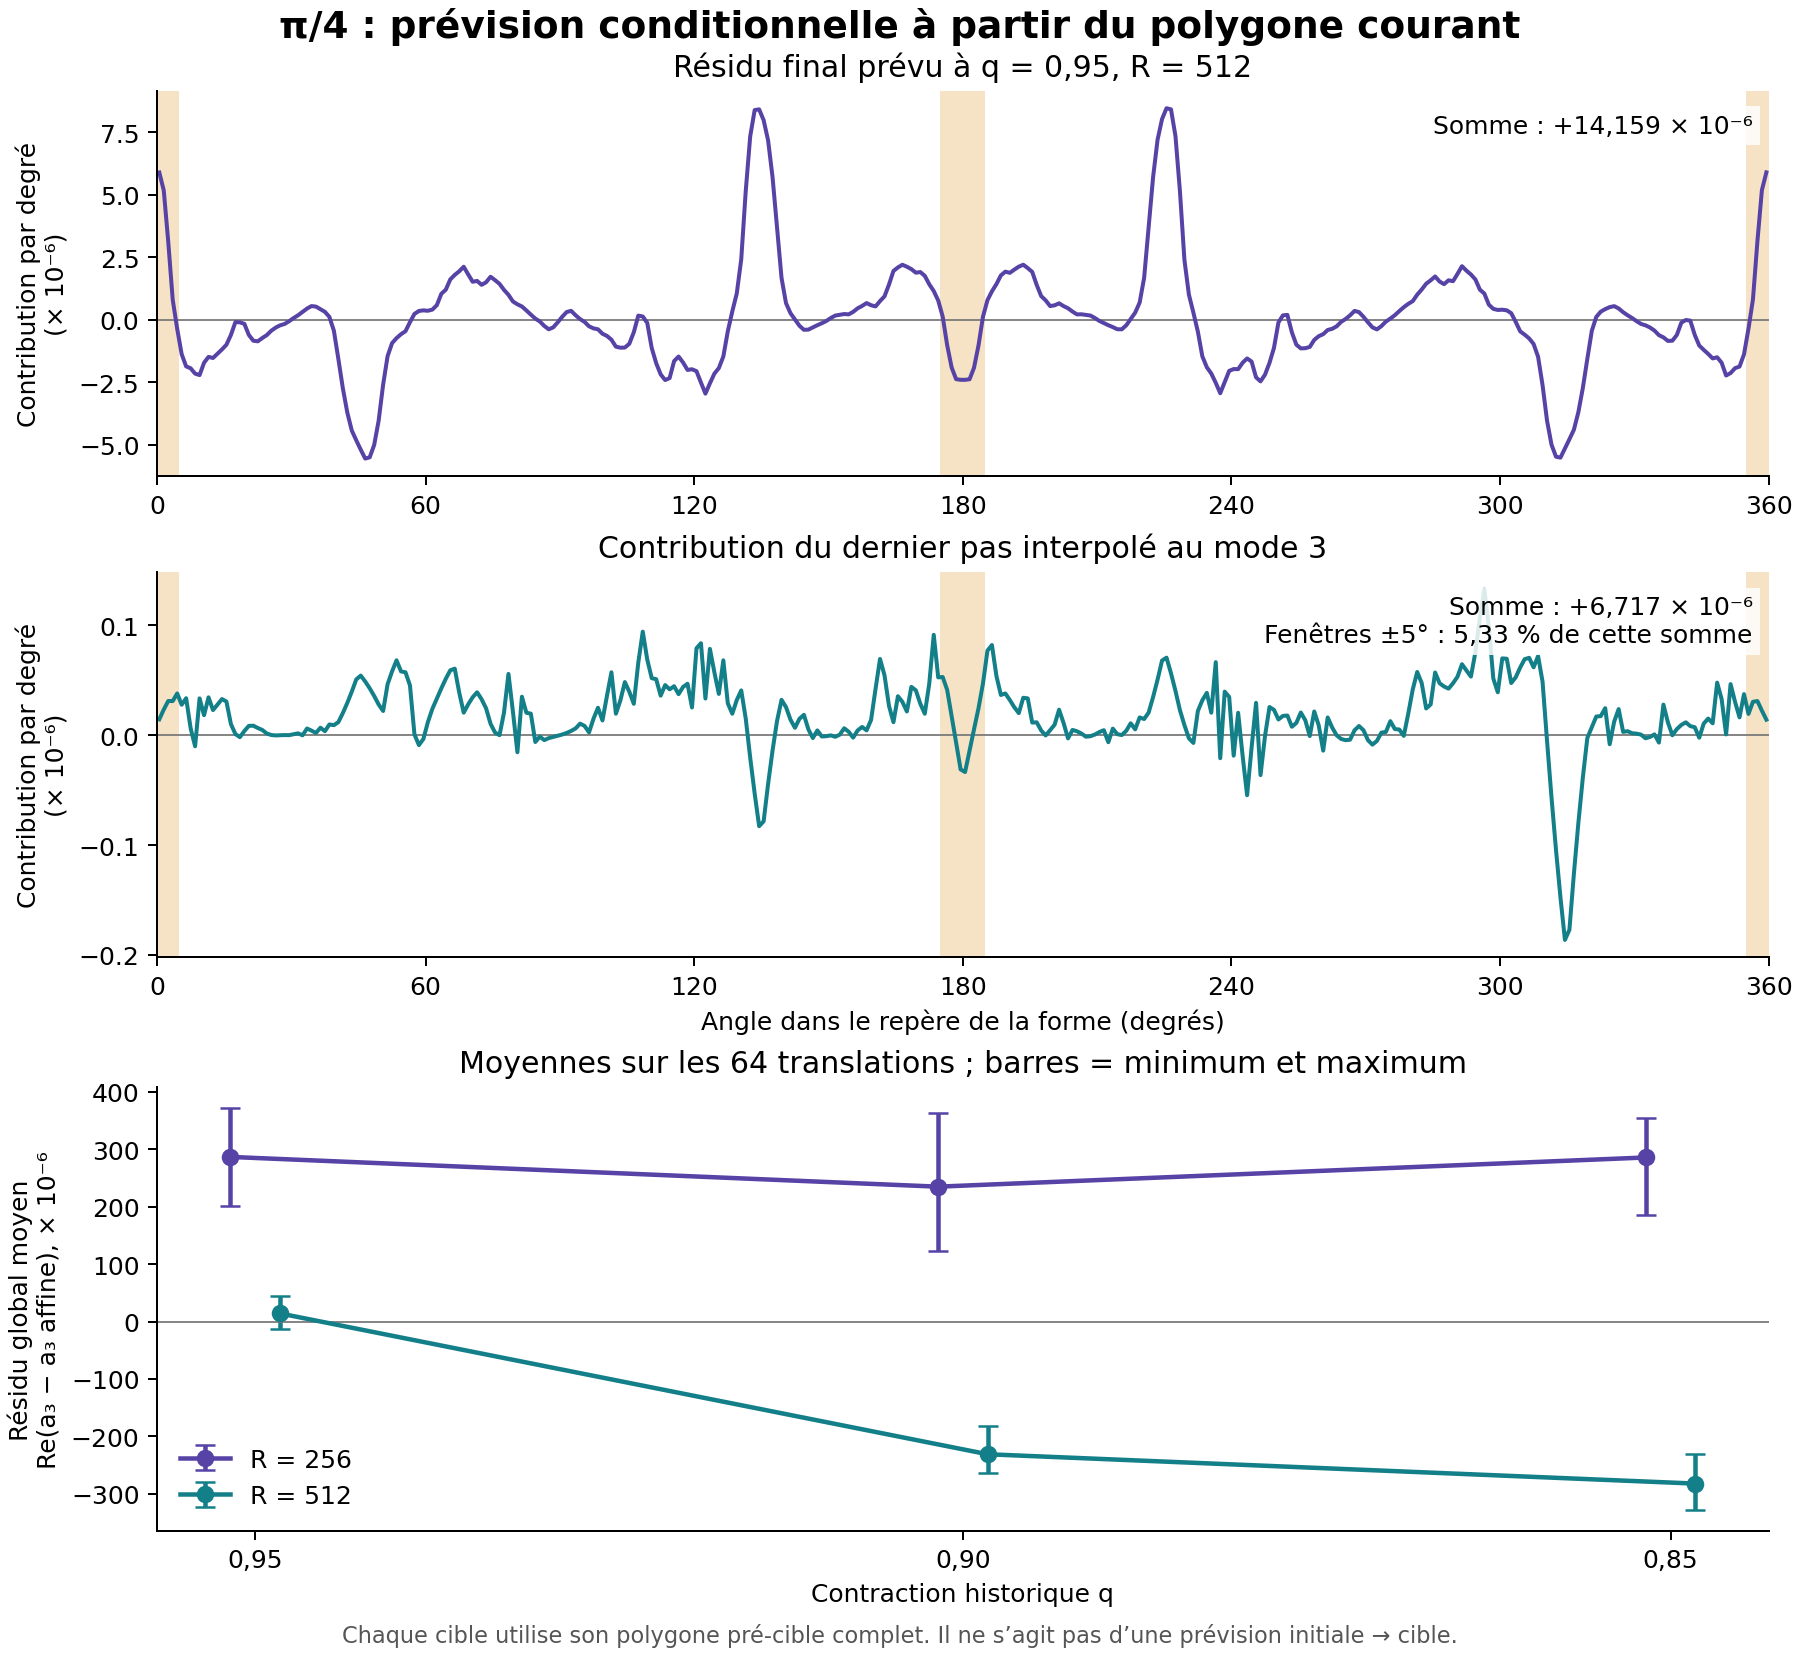
\includegraphics[width=\textwidth,height=0.83\textheight,keepaspectratio]{figure_prediction_pi4.png}
\caption{Prévision conditionnelle à partir du polygone pré-cible complet. Les deux premiers panneaux concernent $R=512$, $q=0{,}95$ et le repère de la forme ; le recentrage est appliqué aux contributions locales. Les fenêtres colorées sont centrées sur $0^\circ$ et $180^\circ$. Les barres du dernier panneau indiquent les extrema des 64 translations, pas un intervalle de confiance.}
\end{figure}
\clearpage
\section{Ce que les seize directions ne déterminent pas}
Nous avons testé deux reconstructions fixées à partir des seize supports observés : l'intersection des demi-plans correspondants et l'interpolation linéaire périodique des écarts à la référence affine. Leur évaluation utilise donc des valeurs connues et constitue un diagnostic de fermeture, non une prévision.

\begin{table}[h]\centering\small
\caption{Diagnostic à $\pi/4$, $R=512$, couche entière supérieure $q095_{\rm upper}$. Cette couche diffère de la cible interpolée des sections précédentes.}
\begin{tabular}{p{0.73\textwidth}r}\toprule
Grandeur moyenne & Valeur\\\midrule
Résidu véritable & $+\sci{1{,}38308}{-5}$\\
Erreur : intersection des seize demi-plans & $+\sci{8{,}63621}{-3}$\\
Erreur : interpolation des écarts de support & $+\sci{1{,}24527}{-4}$\\
Erreur : même interpolation, avec $c_0$ véritable & $+\sci{9{,}42815}{-5}$\\\bottomrule
\end{tabular}
\end{table}

Les erreurs des variantes interpolées dépassent la valeur absolue du résidu dans les 64 configurations concernées. Ce résultat invalide ces reconstructions à l'échelle du signal. Il ne constitue pas une borne inférieure sur l'erreur de tout modèle imaginable.

Pour les supports convexes lisses généraux, un argument distinct montre la non-identifiabilité par seize échantillons, même avec $c_0$ connu. Si $\alpha_j$ sont les directions non orientées, posons $F(\phi)=\prod_j\sin^2(\phi-\alpha_j)$ et $f(\phi)=F(\phi)\cos3\phi$. Alors $f$ s'annule aux directions échantillonnées, son intégrale est nulle par décalage de $\pi$, et $\int f\cos3\phi=\int F\cos^2 3\phi>0$. Pour $\varepsilon$ assez petit, les supports $h_0\pm\varepsilon f$ restent strictement convexes, ont les mêmes échantillons et le même $c_0$, mais des modes 3 différents. Cet argument concerne la classe des supports lisses ; il ne démontre pas une impossibilité propre à notre trajectoire entière déterministe.

\section{Interprétation et limites}
À $\pi/4$, $R=512$, $q=0{,}95$, le dernier pas interpolé apporte $+\sci{6{,}716707}{-6}$ au mode 3. Les deux fenêtres centrées apportent $+\sci{0{,}255081}{-6}$ et $+\sci{0{,}103027}{-6}$, soit 5,33\,\% de cette somme nette. Leur poids proche de 99\,\% dans le résidu net final ne décrit donc pas la localisation du dernier pas. L'état déjà accumulé et les compensations comptent.

Le succès conditionnel utilise toute la géométrie courante et réalise essentiellement un pas du procédé discret. Il établit un transfert exact entre géométrie et observable, sans fermer l'évolution de cette observable seule. La prédiction autonome initiale-cible, un exposant universel, une résonance diagonale, une nouvelle valeur de $\pi$ et une validation physique de la Dynagénèse ne sont pas établis.

\newpage
\section{Reproduction, disponibilité et relecture}
Les suppléments accompagnent les contrôles de symétrie, la localisation angulaire, les déplacements bruts et les prévisions conditionnelles. Ils comprennent les plans datés, les entrées compactes, les scripts, les benchmarks séparés, les résultats, les figures et les manifestes SHA-256. Les originaux figés sont conservés. Les contrôles de symétrie ont nécessité 18 trajectoires supplémentaires, avec les translations figées, sans nouveau tirage ni nouvelle intégration d'EDP. Les analyses ultérieures de localisation et de déplacement réutilisent les trajectoires sauvegardées ; les prévisions conditionnelles calculent des enveloppes à un pas, sans nouvelle campagne autonome de prévision.

Les scripts portables \texttt{run\_amplitude\_checks.py} et \texttt{run\_mode3\_prediction.py} recomposent les vérifications depuis les données compactes. Pour le premier, les populations de sections et le nombre de sommets sur la ligne inférieure sont des mesures extraites et qualifiées ; leur réextraction depuis les 64 NPZ d'origine n'est pas refaite par le replay compact. Le second reconstruit effectivement le prochain polygone depuis chaque état courant fourni.

La qualification des sections comprend la vérification des 64 empreintes sources, des populations de faces et de 631 sections par une autre implémentation entière. Les 1\,152 résidus prévus retrouvent la localisation antérieure à $\sci{2{,}429}{-16}$ près. Les données Windows du mode global et leur archive angulaire ont été contrôlées par leurs empreintes, les agrégats des CSV et les sommes des secteurs. Les résultats du replay Windows du certificat d'amplitude n'ont pas été transmis à ce stade ; les calculs de référence et la preuve du certificat restent disponibles.

Les accords proches de l'arrondi machine ne certifient pas l'erreur de l'EDP continue, ni le prédicat initial en tous points. Les budgets de référence sont numériques et non des encadrements globaux par intervalles. Les analyses locales sont rétrospectives et les mesures d'une même trajectoire sont dépendantes. La nouveauté exacte du certificat élémentaire et de son application requiert une comparaison bibliographique plus large.

La publication initiale est identifiée par le DOI \href{https://doi.org/10.5281/zenodo.23728565}{10.5281/zenodo.23728565} et le dépôt \href{https://github.com/royerpatrick-ops/dyn-validex-grid-peeling-finite-scale}{dyn-validex-grid-peeling-finite-scale}. Le présent PDF n'attribue aucun nouvel identifiant non encore réservé. Les liens et la version de diffusion du complément doivent être inscrits dans les métadonnées de publication après leur création effective.

\textbf{Relecture sollicitée.} Nous sollicitons une expertise en géométrie discrète et en flots de courbure sur quatre points : antériorité du certificat, portée de l'anisotropie observée, suffisance des contrôles de référence et conception d'un état réduit permettant une prévision sur plusieurs couches. Le succès ou l'échec d'un tel modèle serait à établir avant toute revendication de fermeture macroscopique.

\textbf{Assistance IA.} Des systèmes d'IA ont assisté l'analyse, la programmation, les vérifications croisées et la rédaction. Les contrôles algorithmiques présentés ne remplacent pas une expertise humaine externe. Patrick Royer porte la responsabilité de la diffusion ; aucune affiliation, évaluation humaine ou garantie de nouveauté n'est ajoutée.

\begin{thebibliography}{9}\small
\bibitem{harpeled} S. Har-Peled et B. Lidický. \textit{Peeling the Grid}. SIAM Journal on Discrete Mathematics 27(2), 650--655, 2013. \href{https://doi.org/10.1137/120892660}{doi:10.1137/120892660}.
\bibitem{eppstein} D. Eppstein, S. Har-Peled et G. Nivasch. \textit{Grid Peeling and the Affine Curve-Shortening Flow}. Experimental Mathematics 29(3), 306--316, 2020. \href{https://doi.org/10.1080/10586458.2018.1466379}{doi:10.1080/10586458.2018.1466379}. Prépublication arXiv:1710.03960.
\bibitem{rote} G. Rote, M. Rüber et M. Saghafian. \textit{Grid Peeling of Parabolas}. SoCG 2024, LIPIcs 293, 76:1--76:18. \href{https://doi.org/10.4230/LIPIcs.SoCG.2024.76}{doi:10.4230/LIPIcs.SoCG.2024.76}.
\bibitem{royer} P. Royer. \textit{Épluchage de réseau et flots de courbure à taille finie : réplication prospective sur 64 translations appariées}. Publication initiale et suppléments, 2026. \href{https://doi.org/10.5281/zenodo.23728565}{doi:10.5281/zenodo.23728565}.
\end{thebibliography}
\end{document}
